%!TEX root = ../dolgozat.tex
\chapter{Tesztelés}
\label{ch:teszteles}

Ebben a fejezetben a rendszer tesztelését és a tesztek eredményeit mutatom be. A tesztelés célja
kettős volt: egyrészt annak ellenőrzése, hogy a rendszer megfelel-e \aref{sec:kovetelmenyek}.
szakaszban megfogalmazott funkcionális követelményeknek, másrészt annak igazolása, hogy
\aref{sec:biztonsagi_terv}. szakaszban tervezett védelmek a gyakorlatban is működnek. A fejezet
végén a rendszer használatát is bemutatom.

\section{A tesztelés módszere és környezete}

Sommerville felosztását követve a tesztelés több szinten történhet: a fejlesztői tesztelés az
egyes komponenseket, a rendszertesztelés az összeépített rendszert, az elfogadási tesztelés
pedig a felhasználó szempontjából vizsgálja a szoftvert \cite{sommerville2016software}. Munkám
során a hangsúlyt a rendszertesztelésre helyeztem: a teszteket a kész alkalmazáson, annak
külső interfészein (a REST API-n és a Socket.IO kapcsolaton) keresztül végeztem, így azok
ugyanazt a viselkedést ellenőrzik, amelyet a valódi kliens is tapasztal. A teszteket Python
szkriptekben automatizáltam, így azok bármikor, például egy módosítás után, megismételhetők.

A tesztekhez a következő környezetet használtam: Windows 11 operációs rendszer, Python 3.12.10,
Docker Desktop (Docker Engine 29.9.3), a sandboxban \texttt{python:3.11-slim} image (Python
3.11.18). A funkcionális és a felügyeleti teszteknél minden futtatás egy ideiglenes, üres SQLite
adatbázist használt, így a tesztek egymástól és a fejlesztési adatbázistól függetlenek voltak. Ezt
az teszi lehetővé, hogy a szerveroldal az SQLAlchemy révén adatbázis-független (lásd
\aref{sec:technologiak}. szakaszt), az éles PostgreSQL adatbázissal végzett tesztelés azonban a
jövőben ajánlott kiegészítés.

\section{Funkcionális tesztelés}
\label{sec:funkcionalis_teszt}

A funkcionális teszteket a FastAPI tesztkliensével végeztem, amely valódi HTTP-kéréseket küld az
alkalmazásnak, de nem igényel futó szervert. A tesztszkript először létrehoz két oktatói és két
hallgatói fiókot, majd egy vizsgát különböző típusú feladatokkal, végül végigjátssza a teljes
vizsgafolyamatot. A tesztesetek kiválasztásánál nemcsak a helyes működést ellenőriztem, hanem
szándékosan hibás vagy jogosulatlan kéréseket is küldtem, hiszen egy vizsgarendszernél legalább
olyan fontos, hogy mit \textit{nem} enged meg. A 32 teszteset és az eredményük
\aref{tab:funkcionalis_tesztek}. táblázatban látható.

{\small
\begin{longtable}{@{}lp{9.2cm}p{2.0cm}c@{}}
  \caption{A funkcionális tesztek eredménye}\label{tab:funkcionalis_tesztek}\\
  \toprule
  Azon. & Teszteset & Kapott & Eredmény \\
  \midrule
  \endfirsthead
  \toprule
  Azon. & Teszteset & Kapott & Eredmény \\
  \midrule
  \endhead
  \bottomrule
  \endfoot
  T01 & Oktatói regisztráció hibás meghívókóddal & 400 & sikeres \\
  T02 & Oktatói regisztráció helyes meghívókóddal & oktató & sikeres \\
  T03 & Hallgatói regisztráció (alapértelmezett szerepkör) & hallgató & sikeres \\
  T04 & Regisztráció már foglalt e-mail címmel & 400 & sikeres \\
  T05 & Bejelentkezés hibás jelszóval & 401 & sikeres \\
  T06 & Védett végpont hívása érvénytelen tokennel & 401 & sikeres \\
  T07 & Vizsga létrehozása hallgatói fiókkal & 403 & sikeres \\
  T08 & Vizsga létrehozása hibás időablakkal (a vége a kezdés előtt) & 422 & sikeres \\
  T09 & Feladat létrehozása nem létező helyes válaszra mutató megoldókulccsal & 422 & sikeres \\
  T10 & Feladat hozzáadása más oktató vizsgájához & 403 & sikeres \\
  T11 & Az oktatói (megoldókulcsot tartalmazó) vizsganézet lekérése hallgatóként & 403 & sikeres \\
  T12 & Vizsga kitöltése oktatói fiókkal & 403 & sikeres \\
  T13 & A hallgatónak küldött feladatok nem tartalmaznak megoldókulcsot & nincs benne & sikeres \\
  T14 & A határidő a kezdés + időtartam (60 perc) & 3600 mp & sikeres \\
  T15 & Az ismételt indítás ugyanazt a kitöltést adja vissza & azonos & sikeres \\
  T16 & Egyválasztós feladatnál két válasz mentése & 422 & sikeres \\
  T17 & Nem létező válaszlehetőség mentése & 422 & sikeres \\
  T18 & Mentés egy másik hallgató kitöltésébe & 404 & sikeres \\
  T19 & A pontszám nem látható a beadás előtt & nincs & sikeres \\
  T20 & Egyválasztós feladat helyes válasza teljes pontot ér & 5/5 & sikeres \\
  T21 & Több választós feladat: a 3 helyesből 2 jó és 1 rossz jelölés & 2/6 & sikeres \\
  T22 & Rövid válasz: a ,,\texttt{\ \ 3,14\ }'' válasz elfogadva a ,,\texttt{3.14}'' kulcsra & 3/3 & sikeres \\
  T23 & A kifejtős válasz a beadás után javításra vár & javításra vár & sikeres \\
  T24 & Összpontszám a beadás után ($5+2+2+3$) & 12/26 & sikeres \\
  T25 & Válasz módosítása a beadás után & 409 & sikeres \\
  T26 & Kézi pontozás a feladat maximumánál több ponttal & 422 & sikeres \\
  T27 & Kézi pontozás egy másik oktató vizsgájában & 403 & sikeres \\
  T28 & A kézi pontozás után a hallgató látja a pontot és a visszajelzést & 20/26 & sikeres \\
  T29 & CSV export: UTF-8 bájtsorrend-jelző és pontosvessző elválasztó & megfelelő & sikeres \\
  T30 & Mentés a határidő és a türelmi idő lejárta után & 409 & sikeres \\
  T31 & A lejárt kitöltés automatikus lezárása; a korábban mentett válasz pontot ér & lezárva, 5 p & sikeres \\
  T32 & Vizsga indítása a kezdési időpont előtt & 403 & sikeres \\
\end{longtable}
}

Mind a 32 teszteset az elvárt eredményt adta. Külön kiemelném a T21-es és a T31-es esetet. A T21
\mref{sec:pontozas}ban ismertetett részpontozási képletet ellenőrzi: a hat pontos feladatnál a
hallgató a három helyes válaszból kettőt, valamint egy hibás választ jelölt meg, így a pontszáma
$\max(0, (2-1)/3) \cdot 6 = 2$ pont. A T31-es teszthez a kitöltés határidejét közvetlenül az
adatbázisban állítottam a múltba, ezzel szimulálva azt a helyzetet, amikor a hallgató a vizsga
közben bezárja a böngészőt, és többé nem tér vissza. A rendszer a következő lekérdezéskor
lezárta a kitöltést, és a korábban automatikusan elmentett választ értékelte, vagyis a hallgató
munkája nem veszett el.

\section{A sandbox biztonsági tesztelése}
\label{sec:sandbox_teszt}

A kódfuttatás biztonságát úgy ellenőriztem, hogy szándékosan ártó programokat futtattam a
valódi Docker-sandboxban, ugyanazon a függvényen keresztül, amelyet a rendszer a hallgatói
megoldások értékelésére használ. Minden tesztprogram egy-egy fenyegetést valósít meg
\aref{sec:sandbox_elmelet}. szakaszban felsoroltak közül. Az eredményeket és az egyes futtatások
teljes idejét (a konténer indításával és törlésével együtt) \aref{tab:sandbox_tesztek}. táblázat
tartalmazza.

{\small
\begin{longtable}{@{}l>{\raggedright\arraybackslash}p{3.9cm}>{\raggedright\arraybackslash}p{6.2cm}rc@{}}
  \caption{A sandbox biztonsági tesztjeinek eredménye}\label{tab:sandbox_tesztek}\\
  \toprule
  Azon. & Támadás & A rendszer reakciója & Idő & Eredmény \\
  \midrule
  \endfirsthead
  \toprule
  Azon. & Támadás & A rendszer reakciója & Idő & Eredmény \\
  \midrule
  \endhead
  \bottomrule
  \endfoot
  B01 & Végtelen ciklus & időtúllépés az 5 mp-es korlátnál & 5,52 s & védett \\
  B02 & Fork bomb (folyamatok indítása ciklusban) & a 64-es folyamatkorlát miatt az \texttt{os.fork} hibát jelez (\textit{Resource temporarily unavailable}) & 0,66 s & védett \\
  B03 & 1 GB memória lefoglalása & a kernel a folyamatot leállítja (SIGKILL, kilépési kód $-9$) & 1,31 s & védett \\
  B04 & Hálózati kapcsolat egy külső címre & \textit{Network is unreachable} & 0,63 s & védett \\
  B05 & Fájl írása az \texttt{/etc} könyvtárba & \textit{Read-only file system} & 0,46 s & védett \\
  B06 & Végtelen mennyiségű kimenet & a kimenet 64 KB-nál csonkolva, majd időtúllépés & 5,44 s & védett \\
  B07 & A vezérlő környezeti változóinak (kód, tesztek) kiolvasása & a hallgató folyamata nem látja őket & 0,45 s & védett \\
  B08 & Az eredményjelölő (\texttt{\_\_RESULTS\_\_}) kiírása a kimenetre & eredetileg az értékelés rendszerhibával leállt; a javítás után a program kimenete közönséges szövegként jelenik meg (lásd a szöveget) & 0,48 s & javítva \\
  B09 & A vezérlőfolyamat leállítása (\texttt{kill 1}) & \textit{Operation not permitted} & 0,55 s & védett \\
  B10 & A futtató felhasználó lekérdezése & UID és GID: 65534 (\texttt{nobody}) & 0,49 s & megfelelő \\
\end{longtable}
}

A tíz tesztből kilenc igazolta a tervezett védelem működését. A végtelen ciklust és a végtelen
kimenetet az időkorlát állította meg, a fork bombát a folyamatszám-korlát, a memóriafoglalást a
konténer memóriakorlátja. A hálózat és a fájlrendszer elérése nem volt lehetséges, a hallgató
programja pedig nem férhetett hozzá a vezérlő adataihoz, és nem állíthatta le azt. A B03-as
tesztnél érdemes megjegyezni, hogy a memóriakorlát túllépésekor a program nem kap Python
kivételt, hanem a kernel azonnal leállítja; a rendszer ezt futási hibaként értékeli.

A B08-as teszt azonban hibát tárt fel. A vezérlőprogram az eredményeket a kimenete végére, egy
\texttt{\_\_RESULTS\_\_} jelölő után írta ki JSON formátumban, a szerver pedig a jelölő
\textit{utolsó} előfordulását kereste meg a konténer kimenetében. A hallgató programjának kimenete
azonban maga is bekerül ebbe a JSON-ba, így ha a program kiírta a jelölő szövegét, a szerver a
JSON belsejében találta meg az utolsó előfordulást, a feldolgozás meghiúsult, és az értékelés
,,Rendszerhiba'' üzenettel állt le. A hiba a pontszám meghamisítására nem adott lehetőséget, mert a
hallgató kimenete a JSON-ban idézőjelek között, megfelelően kódolva szerepel, így abból érvényes
eredménylista nem állítható elő; a következménye az volt, hogy az érintett válasz pontozatlan maradt.

A hibát két lépésben javítottam. Mivel a vezérlőprogram a jelölő előtt semmit nem ír ki, és a
hallgató kimenete csak a jelölő utáni JSON-ban szerepelhet, a szerver most a jelölő
\textit{első} előfordulását keresi meg. Emellett a jelölő már nem rögzített szöveg: a szerver
minden kiértékeléshez egy véletlenszerű, 128 bites azonosítót tartalmazó jelölőt
(\texttt{\_\_RESULTS\_<véletlen hexa>\_\_}) generál, és azt csak a vezérlőprogram környezeti
változójában adja át. A hallgató programjának környezetébe ez nem kerül át, és a vezérlő
folyamat környezetét (\texttt{/proc/1/environ}) sem olvashatja, így a jelölőt nem ismerheti.
A javítás után megismételt tesztben a jelölő szövegét kiíró program kimenete közönséges
szövegként jelent meg az eredményben, a \texttt{\_\_RESULTS\_\_} szöveget elvárt kimenetként
megadó feladatot pedig a rendszer helyesen, teljes pontszámmal értékelte.

\section{Teljesítmény}
\label{sec:teljesitmeny}

A programozási feladatok értékelésének sebességét két szempontból vizsgáltam. A pontozás
helyességét egy két tesztesetből (egy nyilvános és egy rejtett) álló, tízpontos feladaton
ellenőriztem: a helyes megoldás 10, a hibás 0 pontot kapott, és a hibás megoldás visszajelzésében
a rejtett teszteset bemenete nem jelent meg. Ezután megmértem, hogyan függ az értékelés ideje a
tesztesetek számától (\mref{tab:teljesitmeny}).

\begin{table}[H]
  \centering
  \caption{Egy kiértékelés átlagos ideje a tesztesetek számának függvényében (3 futás átlaga)}
  \label{tab:teljesitmeny}
  \begin{tabular}{@{}rr@{}}
    \toprule
    Tesztesetek száma & Átlagos idő \\
    \midrule
    1  & 0,44 s \\
    10 & 0,76 s \\
    20 & 1,04 s \\
    \bottomrule
  \end{tabular}
\end{table}

Az eredmények igazolják \mref{sec:sandbox}ban leírt tervezési döntést. Egy kiértékelés idejének
nagyobb részét a konténer indítása és törlése teszi ki (kb. 0,4 másodperc), egy-egy további
teszteset pedig csak körülbelül 30 milliszekundummal növeli az időt. Ha minden tesztesethez
külön konténer indulna, egy 20 tesztesetből álló feladat értékelése ennek alapján
nagyságrendileg 8--9 másodpercig tartana az egy konténerrel mért egy másodperc helyett. A mért
idők bőven megfelelnek a követelményeknek, hiszen a hallgató a beküldés után egy másodpercen belül
megkapja az eredményt. Megjegyzendő, hogy a mérés egyetlen felhasználóval, fejlesztői gépen
készült; terheléses tesztelést, vagyis sok egyidejű beküldés vizsgálatát nem végeztem.

\section{A valós idejű felügyelet tesztelése}
\label{sec:felugyelet_teszt}

A felügyelet szerveroldali működését egy futó szerverrel és Python nyelvű Socket.IO kliensekkel
teszteltem, amelyek a hallgatói és az oktatói klienst szimulálták. Az eredményeket
\aref{tab:socket_tesztek}. táblázat tartalmazza.

{\small
\begin{longtable}{@{}lp{8.6cm}p{2.6cm}c@{}}
  \caption{A valós idejű felügyelet tesztjeinek eredménye}\label{tab:socket_tesztek}\\
  \toprule
  Azon. & Teszteset & Kapott & Eredmény \\
  \midrule
  \endfirsthead
  \toprule
  Azon. & Teszteset & Kapott & Eredmény \\
  \midrule
  \endhead
  \bottomrule
  \endfoot
  S01 & Csatlakozás token nélkül & elutasítva & sikeres \\
  S02 & Csatlakozás érvénytelen tokennel & elutasítva & sikeres \\
  S03 & Egy másik oktató belépése a vizsga szobájába & elutasítva & sikeres \\
  S04 & Hallgató belépése folyamatban lévő kitöltés nélkül & elutasítva & sikeres \\
  S05 & Az oktató belépéskor pillanatképet kap a kitöltésekről & megkapta & sikeres \\
  S06 & Az oktató értesítést kap a hallgató belépéséről & megkapta & sikeres \\
  S07 & 10 ablakelhagyás jelzése az oktatónak & 10 riasztás & sikeres \\
  S08 & A szabálysértések száma az adatbázisban is megjelenik & 10 & sikeres \\
  S09 & Beadáskor az oktató értesítést kap & megkapta & sikeres \\
  S10 & A beadás után küldött jelzés figyelmen kívül marad & nincs riasztás & sikeres \\
\end{longtable}
}

Mind a tíz teszteset sikeres volt. Az S07-es tesztben azt is megmértem, mennyi idő telik el a
hallgatói kliens jelzésének elküldése és a riasztás oktatói klienshez érkezése között: tíz mérés
alapján az átlag 8,9 ms volt (legkisebb 8,2 ms, legnagyobb 11,1 ms). A tesztkliens a WebSocket
helyett HTTP hosszú lekérdezéssel kommunikált, a mérés pedig egyetlen gépen, helyi hálózaton
történt, így valós hálózati körülmények között a hálózati késleltetés is hozzáadódik; a riasztás
az oktató számára ennek ellenére gyakorlatilag azonnalinak tekinthető.

A kliensoldali érzékelést, vagyis azt, hogy a böngésző valóban jelzi-e az ablak elhagyását, csak
valódi böngészőben lehet ellenőrizni. A tesztet Windows 11 operációs rendszeren, a Google Chrome
157-es verziójával végeztem. A hallgatói vizsgaoldalt egy önálló Chrome-ablakban nyitottam meg,
és a műveleteket valódi billentyűparancsokkal (\texttt{Ctrl+T}, \texttt{Ctrl+W}, \texttt{Ctrl+L},
\texttt{F5}), illetve az ablak kis méretre állításával és egy másik alkalmazás előtérbe hozásával
hajtottam végre. Minden lépés után összevetettem a hallgatói fejlécben látható ablakváltás-számlálót,
az oktatói oldalon megjelenő értéket és az oldalon kiváltott böngészőesemények sorrendjét. Az
eredményeket \aref{tab:bongeszo_tesztek}. táblázat foglalja össze.

{\small
\begin{longtable}{@{}l>{\raggedright\arraybackslash}p{4.2cm}>{\raggedright\arraybackslash}p{6.4cm}c@{}}
  \caption{A böngészőoldali felügyelet tesztjeinek eredménye}\label{tab:bongeszo_tesztek}\\
  \toprule
  Azon. & Művelet & Kiváltott események & Figyelm. \\
  \midrule
  \endfirsthead
  \toprule
  Azon. & Művelet & Kiváltott események & Figyelm. \\
  \midrule
  \endhead
  \bottomrule
  \endfoot
  K01 & Új lap megnyitása, majd visszatérés a vizsgafülre & \texttt{blur}, \texttt{visibilitychange} (\textit{hidden}), \texttt{visibilitychange} (\textit{visible}), \texttt{focus} & 1 \\
  K02 & Váltás másik alkalmazásra (Alt+Tab) & \texttt{blur} & 1 \\
  K03 & Ablak kis méretre állítása, majd visszaállítása & \texttt{blur}, \texttt{visibilitychange} (\textit{hidden}), \texttt{visibilitychange} (\textit{visible}), \texttt{focus} & 1 \\
  K04 & Az oldal frissítése (F5) & \texttt{pagehide}, \texttt{visibilitychange} (\textit{hidden}) & 0\textsuperscript{*} \\
  K05 & Kattintás a böngésző címsorába & \texttt{blur} & 1 \\
  \multicolumn{4}{@{}l}{\footnotesize\textsuperscript{*}A javítás előtt 1 (lásd a szöveget).}\\
\end{longtable}
}

A fülváltás (K01) és a kis méretre állítás (K03) esetén a böngésző két eseményt is küld az ablak
elhagyásakor: a fókusz elvesztését (\texttt{blur}) és a lap elrejtését (\texttt{visibilitychange}).
A kliens ezeket egyetlen elhagyásnak tekinti, mert az első esemény után egy jelzőt állít be, amelyet
csak az ablak újbóli fókuszba kerülése (\texttt{focus}) töröl; a fülváltás így a tervezettnek
megfelelően egyszer számít. Másik alkalmazásra váltáskor (K02) a lap látható marad, ezért csak a
\texttt{blur} esemény érkezik, ez is egy figyelmeztetést eredményezett. A számláló értéke minden
esetben azonnal megjelent az oktatói monitoron, és megegyezett az adatbázisban tárolt értékkel.

A teszt két olyan esetre is rávilágított, amikor a rendszer a hallgató szándékától függetlenül
jelzett. Az oldal frissítésekor (K04) a böngésző a régi oldal elhagyása előtt elrejtettnek jelöli a
lapot, és a kliens eredetileg ezt is elküldte a szervernek, így minden frissítés egy
figyelmeztetést okozott. A hibát úgy javítottam, hogy a kliens a \texttt{pagehide} eseményre,
vagyis az oldal elhagyásának kezdetére egy jelzőt állít be, és ezután nem küld több figyelmeztetést;
ha a böngésző a vissza gombbal a gyorsítótárból állítja vissza az oldalt (\texttt{pageshow}), a
jelző törlődik. Az oldal elhagyása így sem marad észrevétlen, mert a Socket.IO-kapcsolat ilyenkor
megszakad, és az oktatói monitor a hallgatót kilépettként jelzi. A javítás után megismételt
tesztben három egymást követő frissítés sem okozott figyelmeztetést, a fülváltás és a kis méretre
állítás viszont továbbra is egy-egy figyelmeztetést eredményezett, a frissítés után is. A
számláló értéke a frissítéskor nem nullázódik, mert a kliens a szervertől kapja vissza a tárolt
értéket.

A böngésző címsorába kattintás (K05) szintén elveszi a fókuszt az oldaltól, ezért figyelmeztetésnek
számít. Ezt a böngésző eseményei alapján nem lehet megkülönböztetni attól, amikor a hallgató egy
másik alkalmazásra vált, ezért ezen nem változtattam. Mivel ilyenkor a hallgató valójában nem
hagyta el a vizsgát, az oktatónak a figyelmeztetések számát nem önmagában, hanem a többi
körülménnyel együtt érdemes értékelnie.

\section{Az alkalmazás használata}
\label{sec:hasznalat}

Ebben a szakaszban röviden, a felhasználó szemszögéből mutatom be a rendszer használatát. A
telepítés lépéseit a dolgozat végén található adathordozó-útmutató tartalmazza.

\paragraph{Oktatóként.} Az oktató a regisztrációs űrlapon az ,,Oktatóként regisztrálok''
lehetőséget választva, a meghívókód megadásával hozhat létre fiókot. Bejelentkezés után az oktatói
felületen új vizsgát hozhat létre, megadva a címét, a leírását, a kezdési és záró időpontot,
valamint a kitöltésre szánt időt. A vizsga oldalán három fül található. A \textit{Feladatok} fülön
adhatók hozzá a feladatok; az űrlap a kiválasztott feladattípushoz igazodik, programozási
feladatnál például a tesztesetek bemenete, elvárt kimenete és láthatósága adható meg. Az
\textit{Élő monitor} fülön a vizsga ideje alatt az oktató látja, mely hallgatók vannak éppen
jelen, hányszor hagyták el a vizsgaablakot, és ki adta már be a dolgozatát. Az
\textit{Eredmények} fülön hallgatónként áttekintheti a válaszokat, pontozhatja a kifejtős
feladatokat, felülírhatja az automatikus pontszámot, szöveges visszajelzést írhat, és az
eredményeket CSV fájlba exportálhatja.

\paragraph{Hallgatóként.} A hallgató a regisztráció és a bejelentkezés után a műszerfalon látja az
elérhető vizsgákat, a vizsgák időpontját, a feladatok számát és az elérhető pontszámot. A vizsga
elindítása után a képernyő tetején rögzített fejléc mutatja a hátralévő időt, a felügyeleti
kapcsolat állapotát (,,Felügyelet aktív'') és az eddigi ablakváltások számát; alatta egy
gombsorban választhatók ki a feladatok, ahol pipa jelzi a már megválaszoltakat. A válaszok
gépelés közben automatikusan mentődnek. Programozási feladatnál a hallgató a kódját a
,,Próbafuttatás'' gombbal kipróbálhatja a nyilvános példatesztekkel vagy saját bemenettel, a
,,Beküldés \& értékelés'' gombbal pedig az összes tesztesettel értékeltetheti, és azonnal látja,
hány teszt volt sikeres. A ,,Vizsga beadása'' gomb megnyomása után -- illetve az idő lejártakor
automatikusan -- a vizsga lezárul, és a hallgató megtekintheti az eredményét.

Az oktatói felület kezdőoldalát \aref{fig:oktatoi_muszerfal}. ábra mutatja: bal oldalon az oktató
vizsgái láthatók az állapotukkal (,,Hamarosan'', ,,Folyamatban''), jobb oldalon az új vizsga
létrehozására szolgáló űrlap. A feladatszerkesztőt, az élő monitort és az eredmények részletes
nézetét \aref{sec:felulet}. szakaszban mutattam be
(\mref{fig:feladatszerkeszto}, \mref{fig:elo_monitor}, \mref{fig:eredmenyek_reszletes}).

\begin{figure}[H]
  \centering
  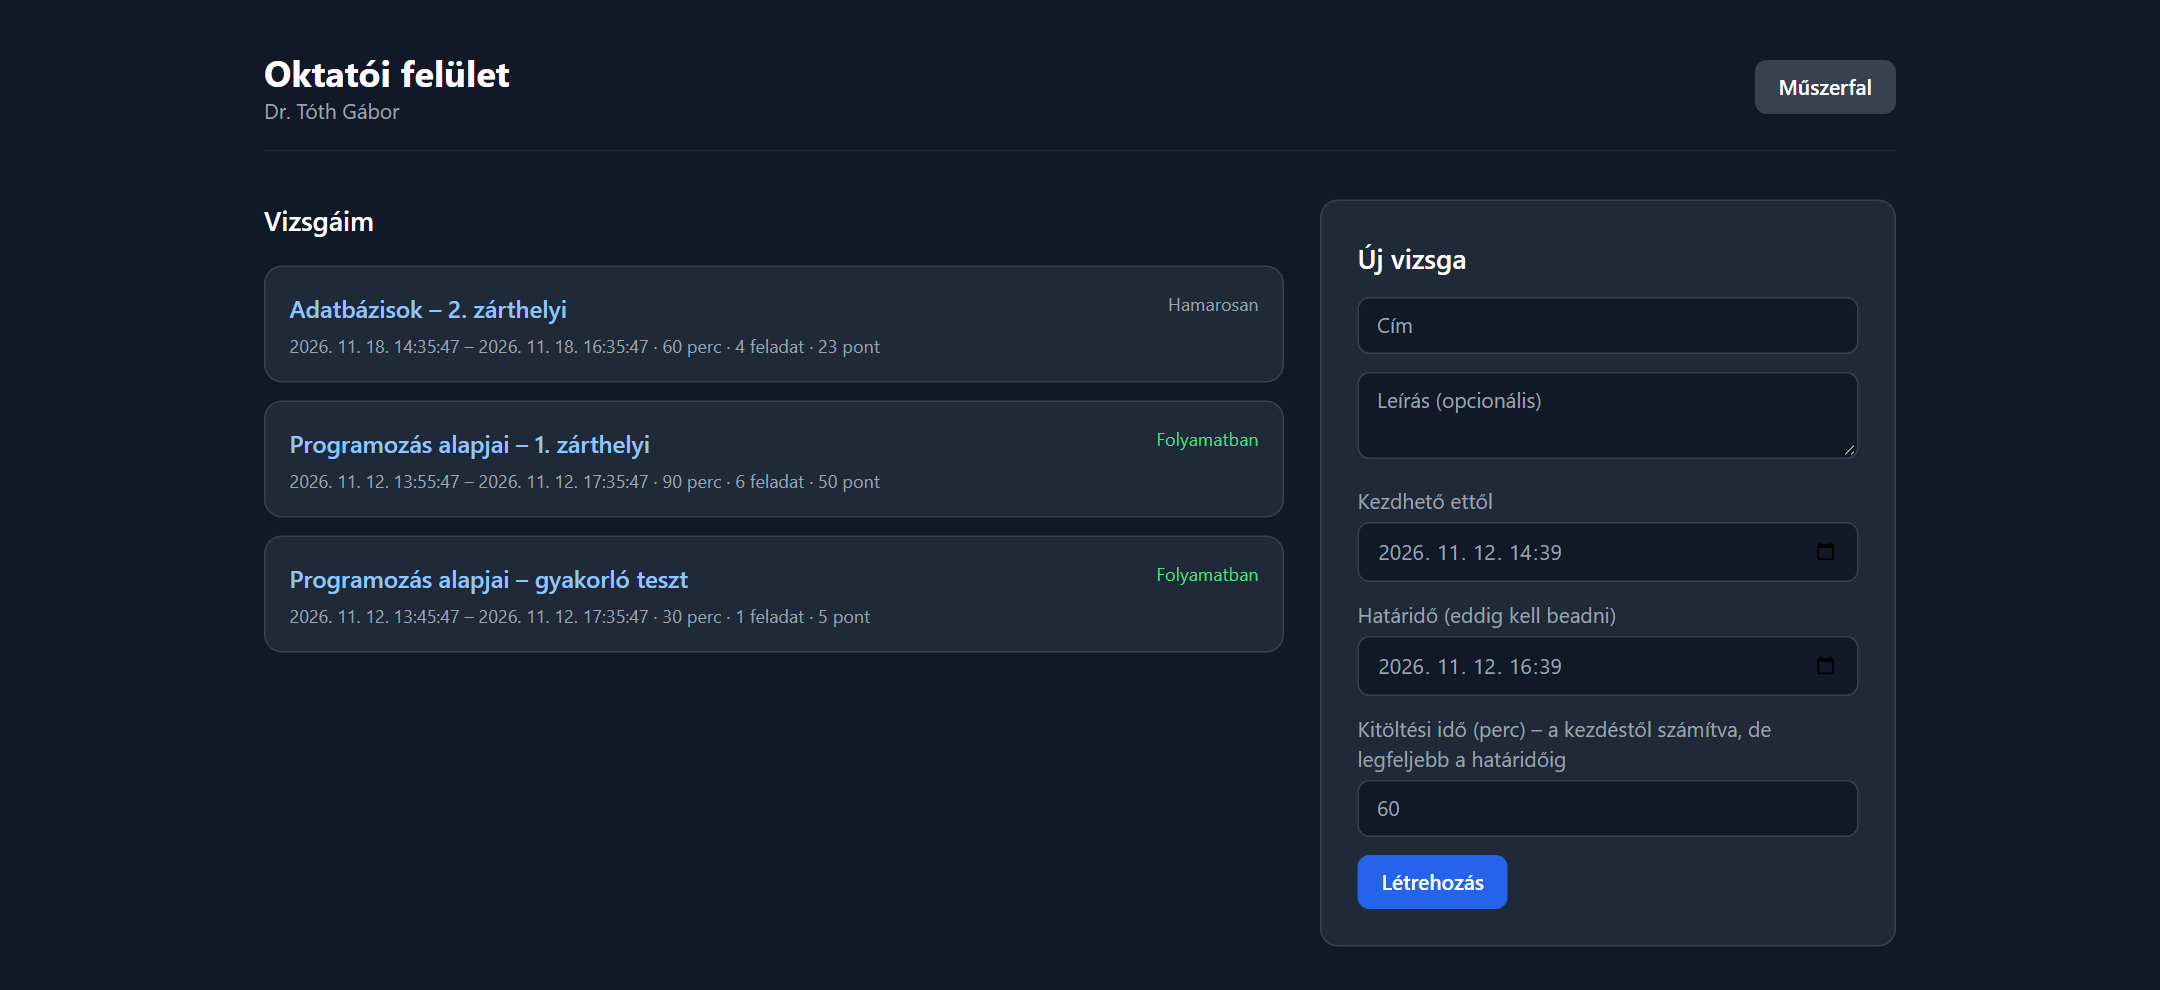
\includegraphics[width=\textwidth]{images/oktatoi_muszerfal.png}
  \caption{Az oktatói felület a vizsgák listájával és az új vizsga űrlapjával}
  \label{fig:oktatoi_muszerfal}
\end{figure}

Az eredmények fül összesítő nézetében (\mref{fig:eredmenyek}) a hallgatók egy-egy sorban
szerepelnek a kezdés és a beadás időpontjával, az ablakváltások számával és a pontszámukkal. A
lista felett a kitöltések száma, az átlagpontszám és a még javításra váró válaszok száma látható,
itt érhető el a CSV export és az újraértékelés is.

\begin{figure}[H]
  \centering
  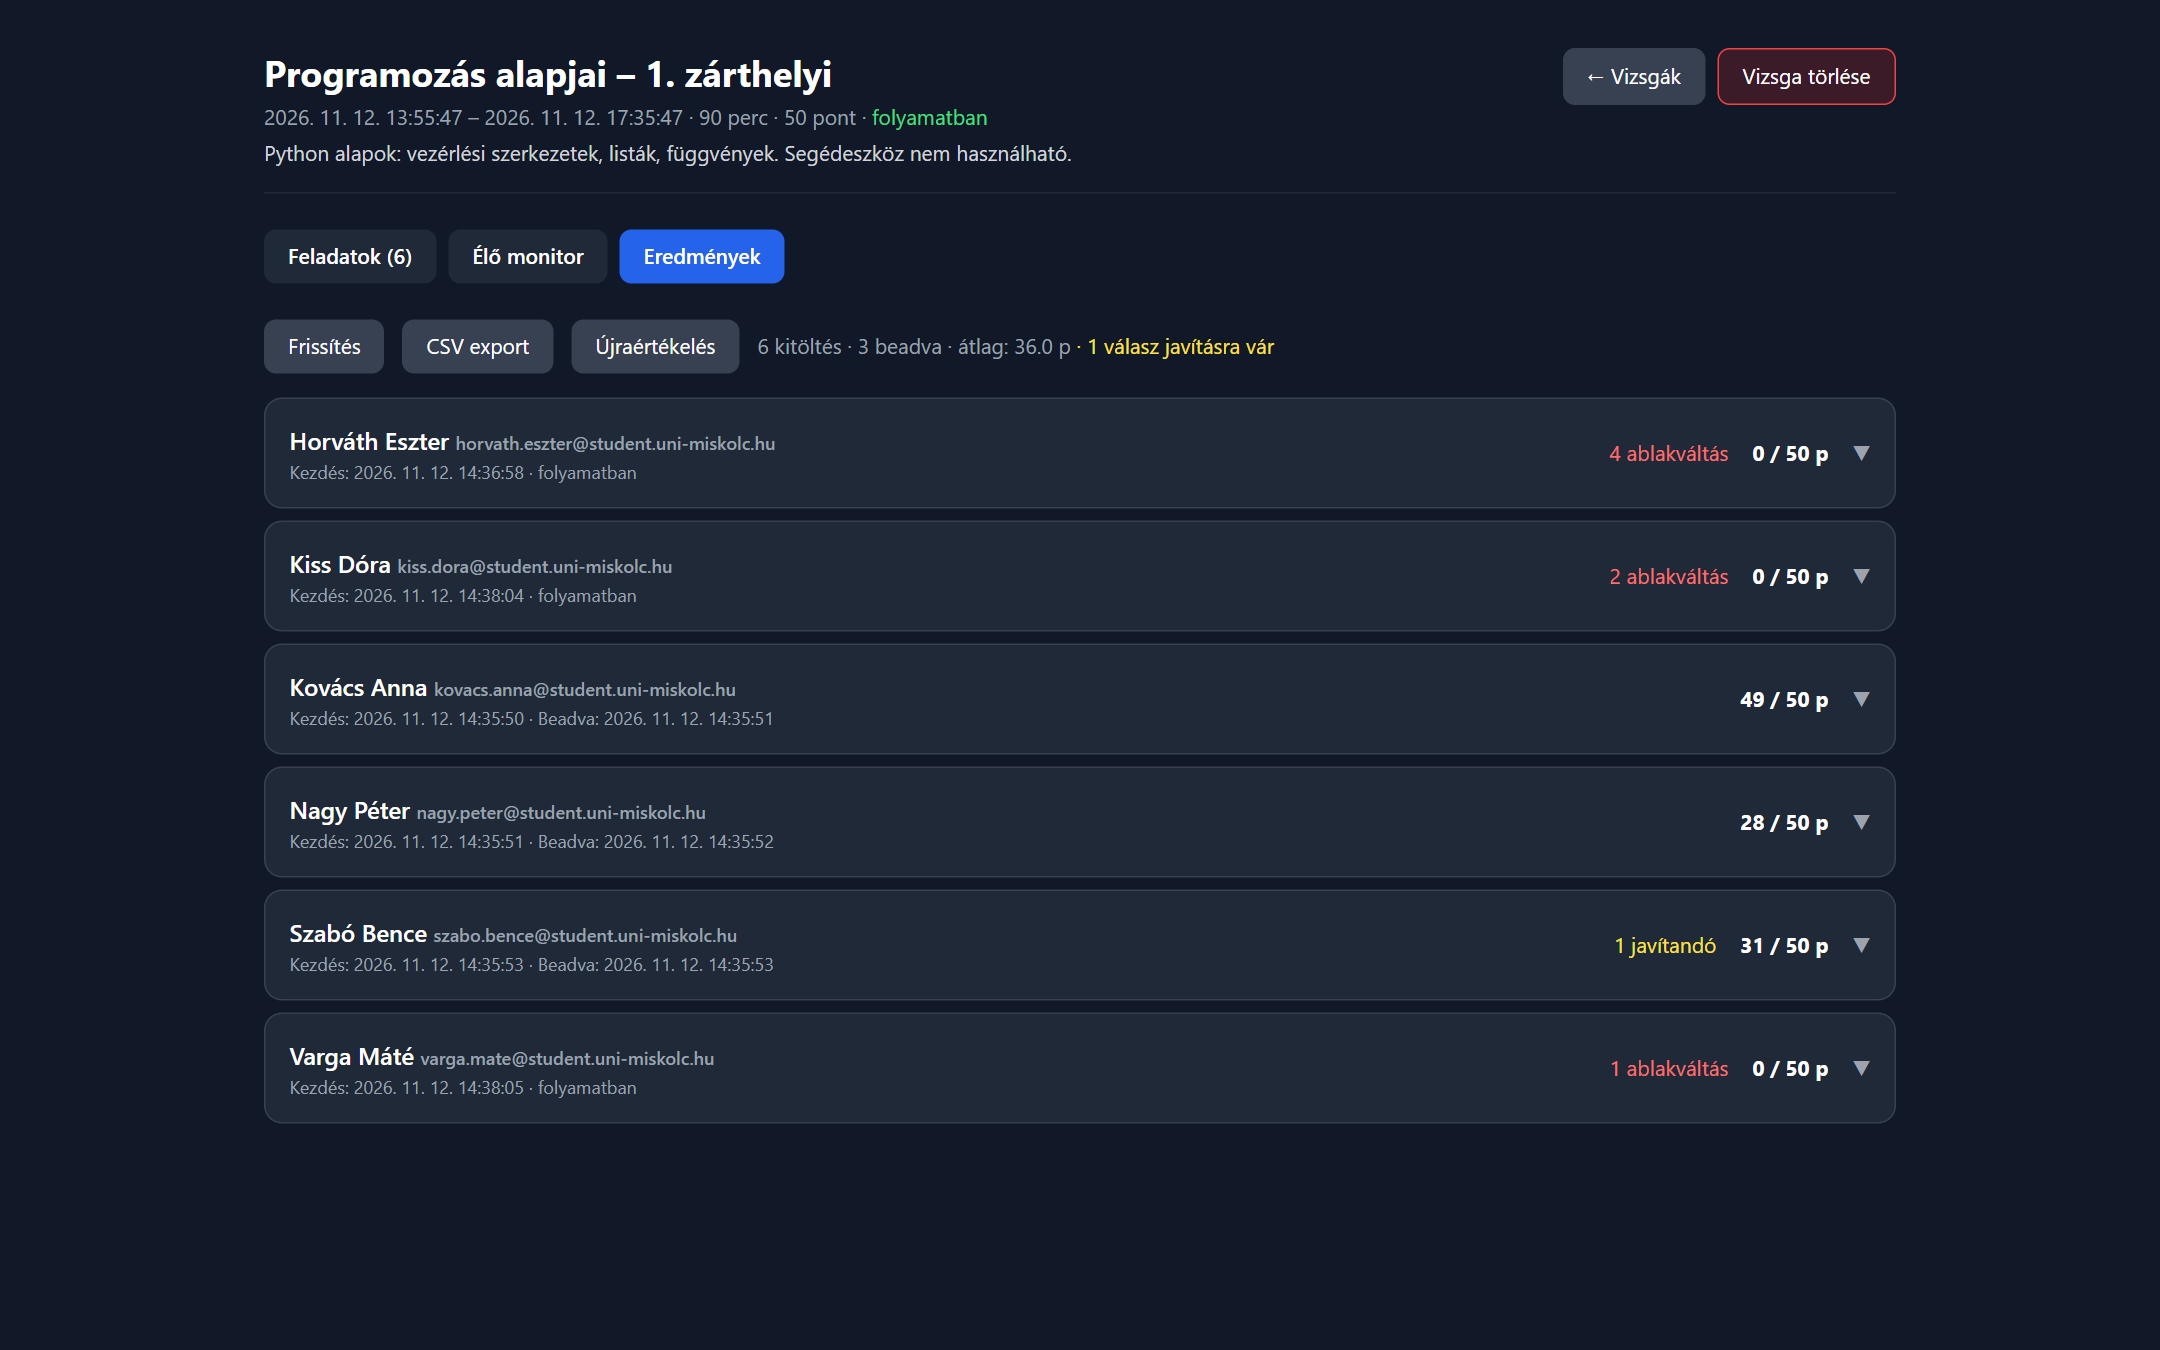
\includegraphics[width=\textwidth]{images/eredmenyek.png}
  \caption{Az eredmények fül összesítő nézete}
  \label{fig:eredmenyek}
\end{figure}

A hallgatói műszerfalat \aref{fig:hallgatoi_muszerfal}. ábra mutatja. Minden vizsga külön kártyán
jelenik meg; a kártya alján lévő gomb az állapottól függően a vizsga indítására, folytatására vagy
az eredmény megtekintésére szolgál, a már beadott és értékelt vizsgáknál pedig a pontszám is
látható.

\begin{figure}[H]
  \centering
  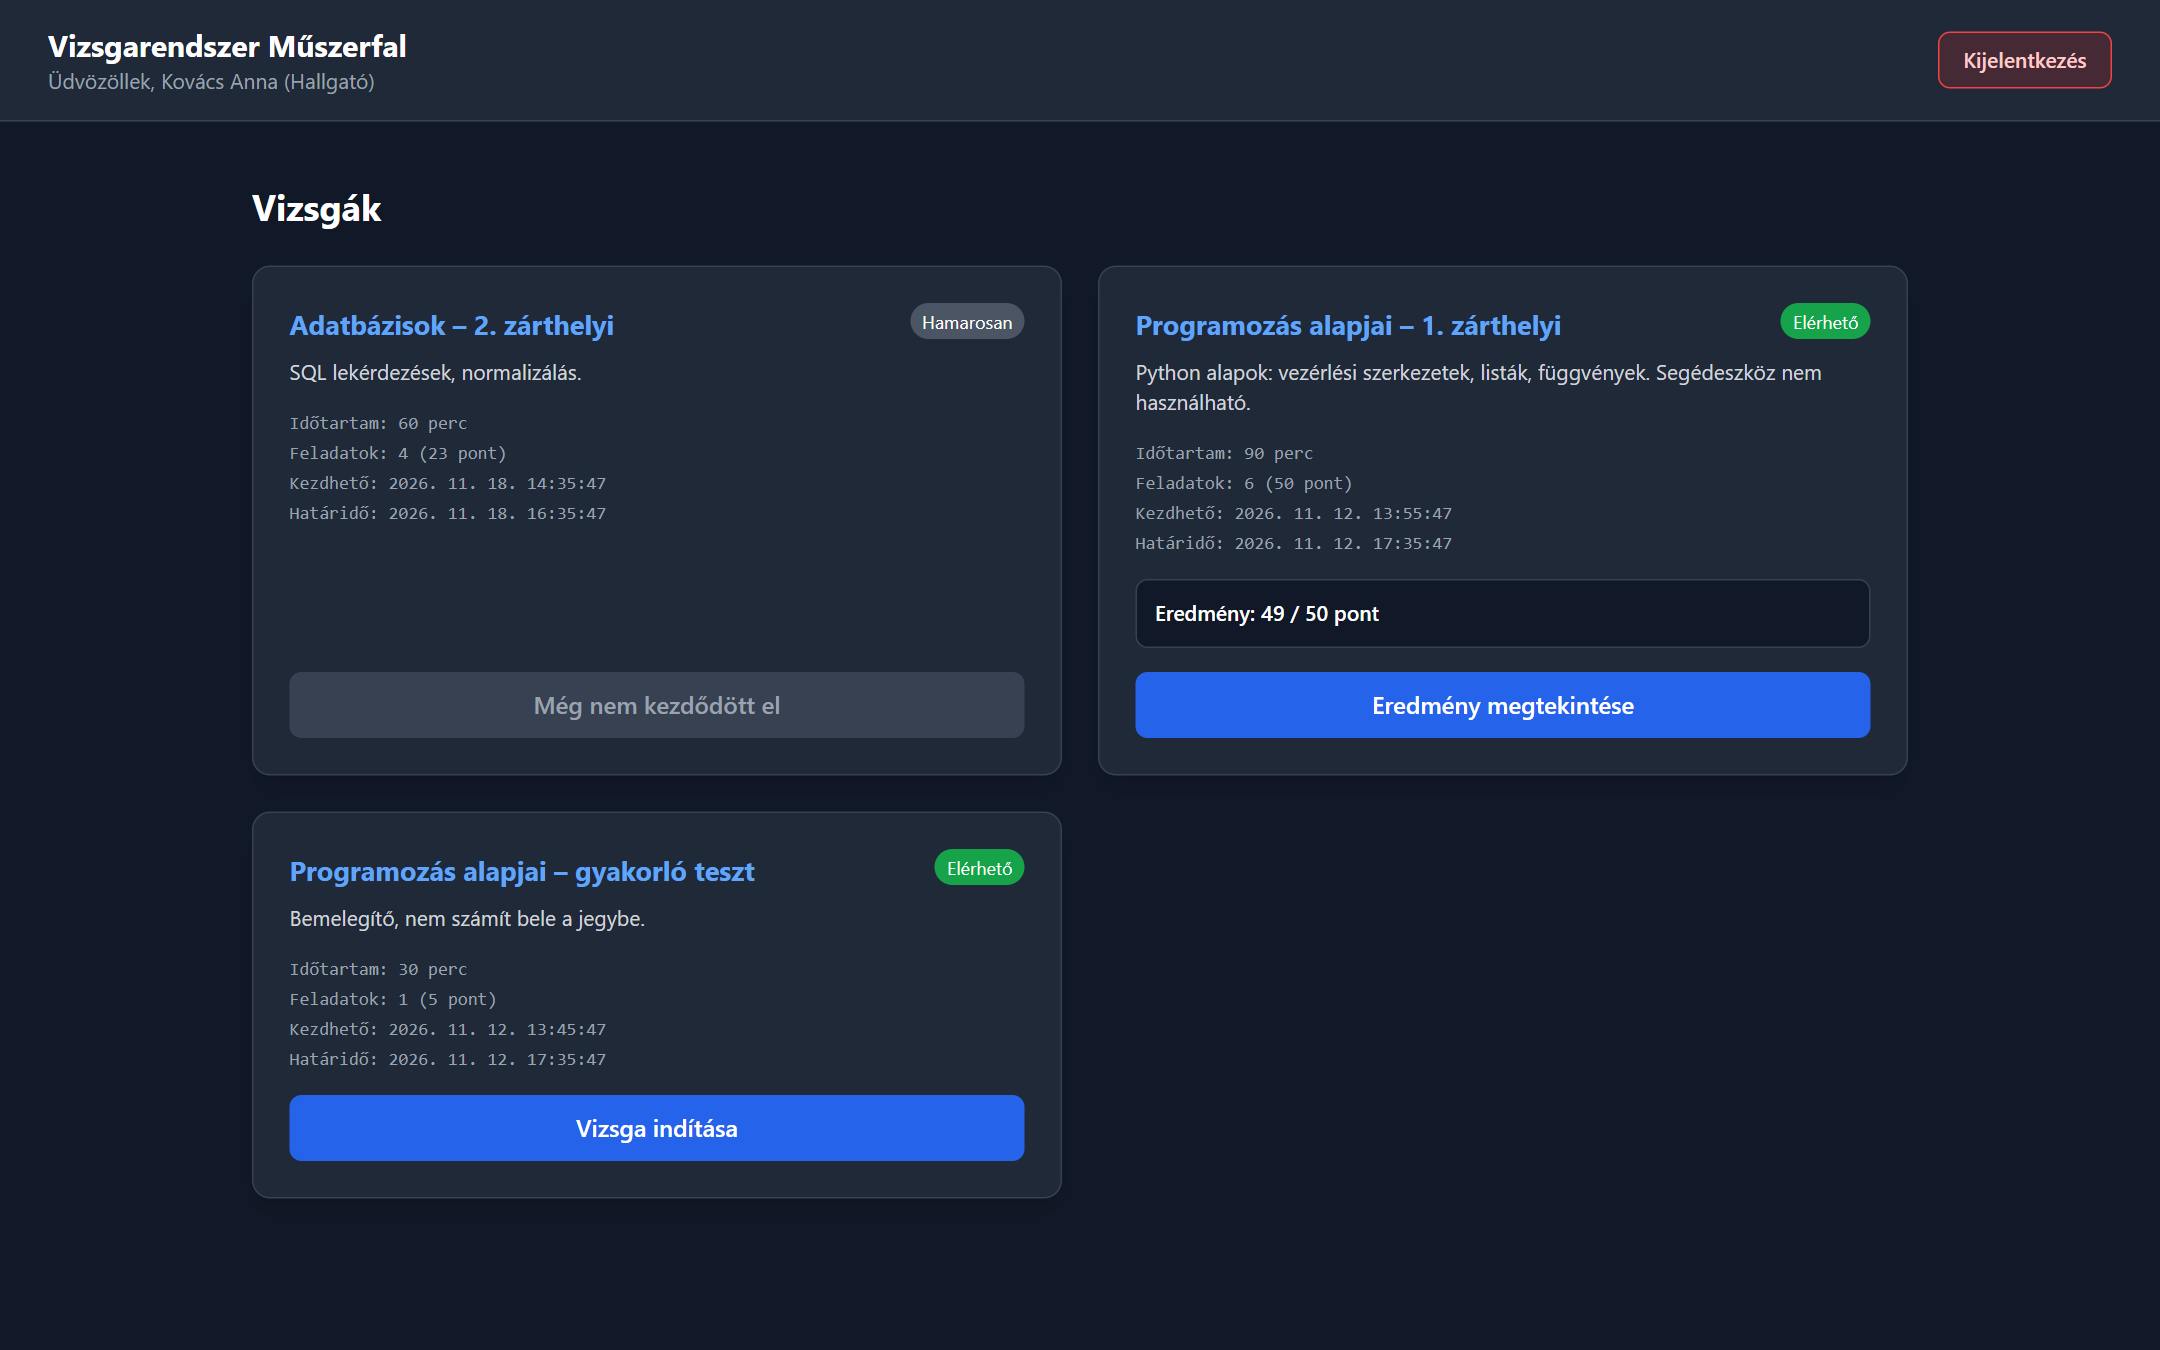
\includegraphics[width=\textwidth]{images/hallgatoi_muszerfal.png}
  \caption{A hallgatói műszerfal}
  \label{fig:hallgatoi_muszerfal}
\end{figure}

A vizsgaoldalt programozási feladattal \aref{fig:vizsgaoldal_kod}. ábra mutatta, választós
feladatnál a válaszlehetőségek jelölőnégyzetekként jelennek meg (\mref{fig:vizsgaoldal_valasztos}).
Több helyes válasz esetén a feladat szövege alatt figyelmeztetés jelzi, hogy a hibás jelölés
pontlevonással jár.

\begin{figure}[H]
  \centering
  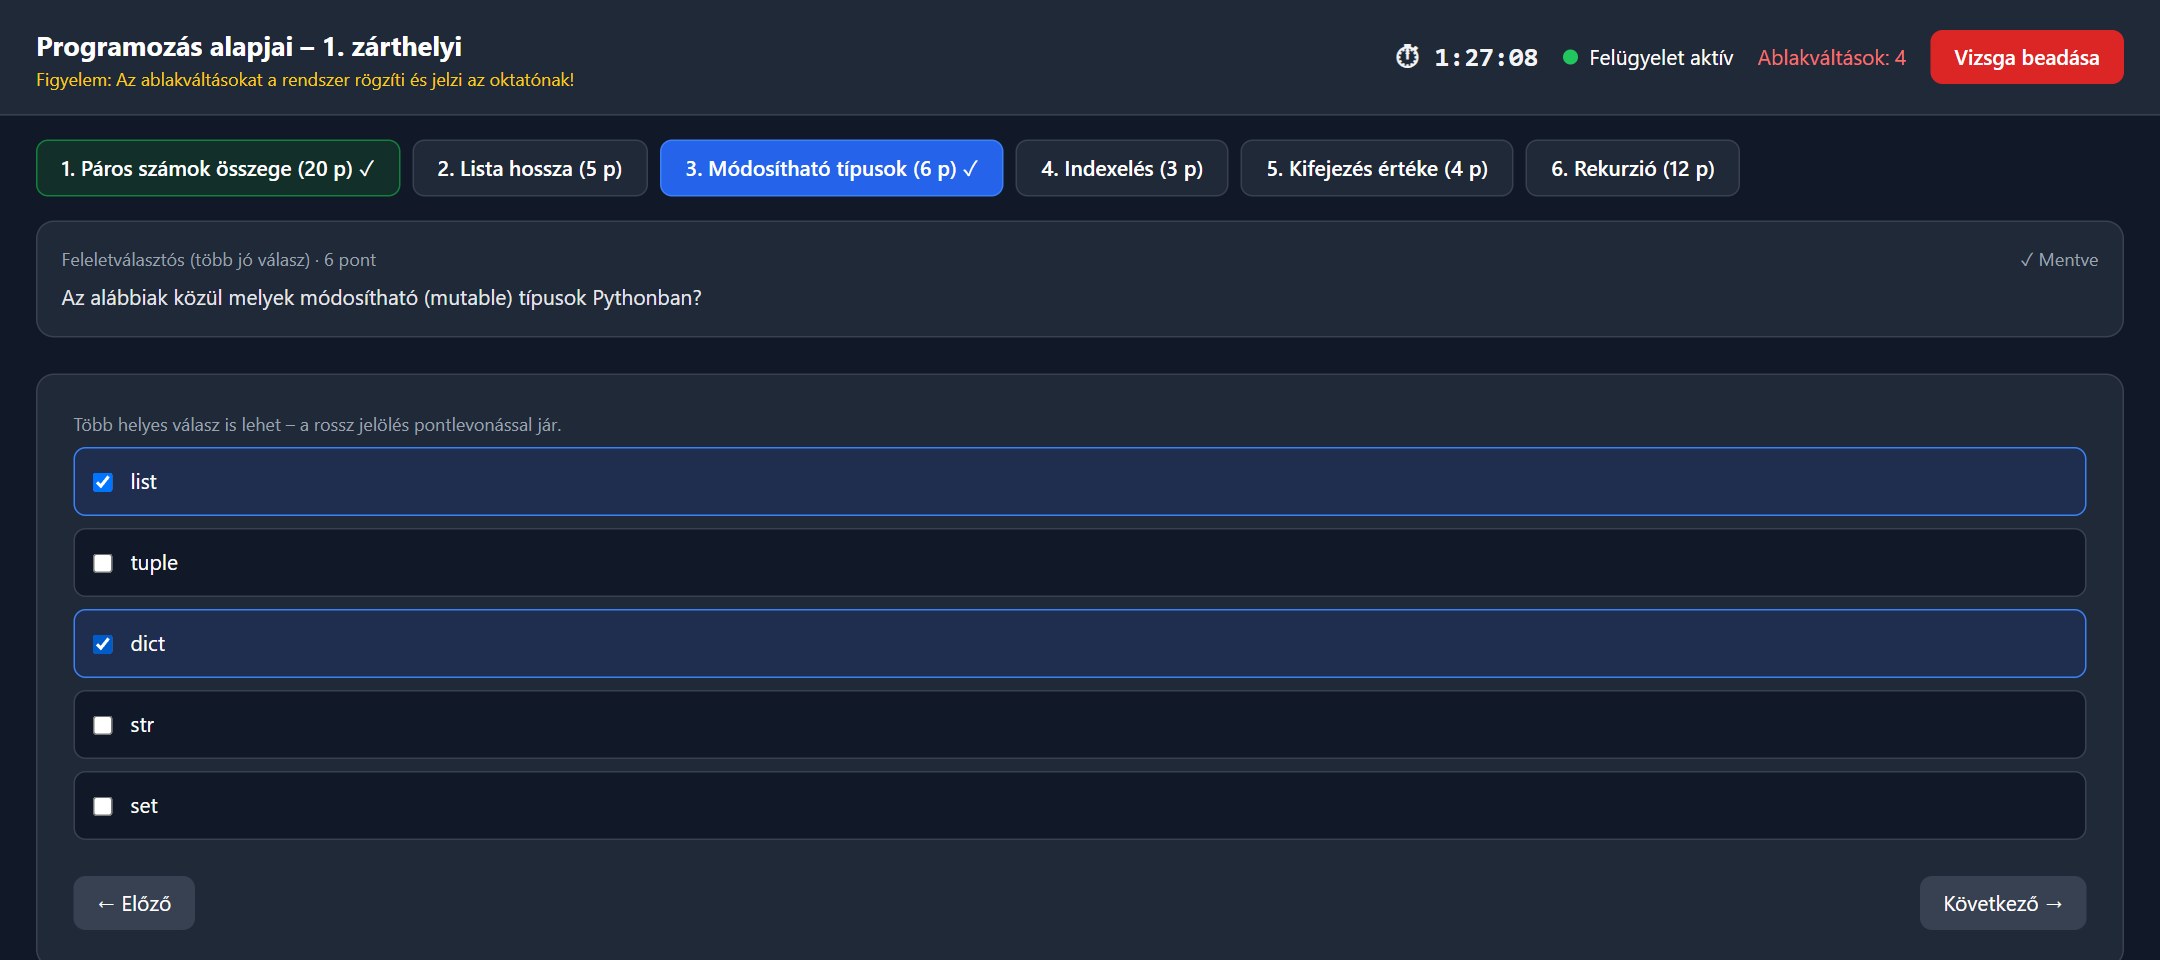
\includegraphics[width=\textwidth]{images/vizsgaoldal_valasztos.png}
  \caption{Több helyes választ tartalmazó feladat a hallgatói vizsgaoldalon}
  \label{fig:vizsgaoldal_valasztos}
\end{figure}

\section{Korlátok}
\label{sec:korlatok}

A tesztelés során a rendszer korlátai is világossá váltak. A kódfeladatok jelenleg csak Python
nyelven oldhatók meg, és az értékelés a kimenet szöveges egyezésén alapul, így a feladatkiírásnak
pontosan meg kell határoznia a kimenet formátumát. A böngészőalapú felügyelet egy második eszköz
használatát nem érzékeli, és egy hozzáértő hallgató a böngésző fejlesztői eszközeivel a jelzések
küldését is megakadályozhatja; a felügyelet tehát az oktató tájékoztatását szolgálja, nem
bizonyítékot szolgáltat. A kódértékelés szinkron módon fut, és a teljes futás idejére lefoglal egy
szálat a szerver szálkészletéből, ezért sok egyidejű beküldés esetén a szerver terhelhetősége
korlátozott lehet; ezt terheléses teszttel nem vizsgáltam. Ezek a korlátok egyben a továbbfejlesztés irányait is kijelölik, amelyekre az
összefoglalásban térek ki.
